\section{Omniprediction for single quantile level forecasts}\label{sec:single_q}

% This section provides an algorithm for omniprediction of single $\alpha$-level quantile level forecasts under online settings. The goal is to come up with $\hat{P}_t$ that minimizes the following omniprediction objective:
% \begin{align}\label{eq:omni_objective_single_q}
%   \sup_{S \in S_\alpha,\, f \in \cf} \frac{1}{T} \sum_{t=1}^T \E_{p \sim \hat{P}_t} [S(p, Y_t)] - \E[S(f(t), Y_t)],
% \end{align}
% where $S_\alpha$ is the class of \textit{all} scoring functions that are consistent for the $\alpha$-level quantile functional and $\cf$ is a set of comparators. comparators can also viewed as base forecasters that provide $\alpha$-level quantile forecasts. Then, the predictions $\hat{P}_t$ can be viewed as (randomized) $\alpha$-level quantile forecast that minimizes all consistent scoring functions, with respect to given base forecasters $\cf$. This can also be viewed as an implicit ensemble of base forecasters $\cf$.
% To minimize the objective \eqref{eq:omni_objective_single_q}, we introduce a variant of Algorithm \ref{alg:omni-twoplayer}. 

% Algorithm \ref{alg:omni-twoplayer_online} shows the high-level idea of the algorithm. At each time $t$, the algorithm solves a minimax program and outputs a probability distribution $\hat{P}_t$ (distributed over two consecutive grid points) as a $\alpha$-level quantile forecast. Then, the algorithm updates the weights $w_{ib}$ to account for which loss function we should care more in next iteration.

% While Algorithm \ref{alg:omni-twoplayer} takes the best comparator for each elementary score $S_\theta$ as input, Algorithm \ref{alg:omni-twoplayer_online_q} takes all predictions made by comparators as input, and the best comparator for each elementary score $S_{\alpha, i}$ is discovered and updated inside the algorithm. This removes the requirement of additional hold-out set for selecting the best comparator. To do so, Algorithm \ref{alg:omni-twoplayer_online_q} considers the set of comparators $\cf=\{f_b\}_{b=1}^F$ to be finite. That said, the algorithm can be easily modified to a version that accommodates more general $\cf$, that takes the best comparator for each elementary score $S_{\alpha, i}$ pre-computed outside the algorithm. .

% More details will follow throughout this section. In Section \ref{subsec:decomp_single_q}, we discuss the decomposition of $S_\alpha$ into a set of elementary scores $S_{\alpha, i}$, $i \in \{0, \ldots, m-1\}$. In Section \ref{subsec:discretization}, we discuss the discretization of $S_\alpha$, predictions, and forecasts that induces low (no) discretization error. Lastly, in Section \ref{subsec:omni_single_q}, we provide a closed-form solution for the minimax program and put the ingredients together and introduce the omniprediction algorithm for single $\alpha$-level quantile forecasts.


This section presents an algorithm for omniprediction of a single $\alpha$-level quantile. The goal is to construct predictions $\hat{P}_t$ that minimize the following omniprediction objective:
\begin{align}\label{eq:omni_objective_single_q}
  \sup_{S \in S_\alpha,\, f \in \cf} \frac{1}{T} \sum_{t=1}^T \E_{p \sim \hat{P}_t} [S(p, Y_t)] - \E[S(f(t), Y_t)],
\end{align}
where $S_\alpha$ denotes the class of \textit{all} scoring functions that are consistent for the $\alpha$-level quantile functional, and $\cf$ is a finite set of comparators. These comparators can be viewed as base forecasters that provide $\alpha$-level quantile predictions. Accordingly, the outputs $\hat{P}_t$ can be interpreted as (randomized) implicit ensemble of the base forecasters that perform well across all consistent scoring functions. \smallskip

To minimize the objective in \eqref{eq:omni_objective_single_q}, we introduce a variant of Algorithm~\ref{alg:omni-twoplayer}. Algorithm~\ref{alg:omni-twoplayer_online} outlines the high-level procedure. At each time step $t$, the algorithm solves a minimax problem and outputs a probability distribution $\hat{P}_t$ (supported on one or two consecutive grid points) as an $\alpha$-level quantile forecast. The weights $w_{ib}$ are then updated to reflect which loss functions should be emphasized in the next iteration. It's worth noting that Algorithm \ref{alg:omni-twoplayer_online} is different in its style from Algorithm \ref{alg:omni-twoplayer} in how to discover the best base forecaster for each elementary score. Instead of having $\sup_{f\in \cf}$ inside the minimax program, Algorithm \ref{alg:omni-twoplayer_online} computes a weighted sum of losses from each base forecaster and update the weights every time step. Although we mainly focus on finite $\cf$ here, infinite $\cf$ can also be accommodated by using a hold-out set approach as \cite{isaac2025omni} proposes. The modified version that accommodates more general $\cf$ can be found in Appendix \ref{appsec:diff_omni_algos}. \smallskip

The remainder of this section provides the necessary components in detail. In Section~\ref{subsec:decomp_single_q}, we present a prior work on the decomposition of $S_\alpha$ into a set of elementary scores $S_{\alpha, i}$ for $i \in [m]$. This simplifies our task of minimizing loss over all consistent scoring functions into minimizing loss over a one-dimensional set of score functions. In Section~\ref{subsec:discretization}, we discuss the discretization of predictions and forecasts, showing that such discretization allows no approximation error when approximating any element in $S_\alpha$ as a weighted sum of elementary scores. Finally, in Section~\ref{subsec:omni_single_q}, we derive a closed-form solution to the minimax problem and combine these ingredients to present the omniprediction algorithm for single $\alpha$-level quantile forecasts.




\begin{algorithm}[h]
  \caption{Online version of two-player game method} \label{alg:omni-twoplayer_online}
  \begin{algorithmic}[1]
  \State \textbf{Data:} Data stream $\{Y_t\}_{t=1}^T$, Grid size $m \in \mathbb{N}$, Learning rate $\eta > 0$, Base forecasters $\cf = \{f_b\}_{b=1}^{B}$.
  \State \textbf{Initialize:} $w_{ib}(1) = \frac{1}{mB}$, for all $i \in [m], b \in [B]$;
  \For{$t = 1, \ldots, T$}
  \State \textbf{1) Make prediction at time $t$}:
  \begin{align*} %\label{eq:minimax_Pt_single_q}
  \hat{P}(t) = \arg\min_{P \in \Delta_m} \max_{P_y \in \Delta_m} \sum_{i=1}^m \sum_{b=1}^B w_{ib}\E_{p\sim P, Y \sim P_y}[S_{\alpha, i}(p,Y) - S_{\alpha, i}(f_b(t),Y)];
  \end{align*}
  \State \textbf{2) Update the weights $w_{ib}$}:
  \[
  w_{ib}(t+1) \propto w_{ib}(t) \exp\bigl(\eta \big(\mathbb{E}_{p \sim \hat{P}(t)}[S_{\alpha, i}(p, Y_t)] 
  - S_{\alpha, i}(f_b(t), Y_t)\big)\bigr), \quad \forall i \in [m], b \in [B];
  \]
  \EndFor
  \end{algorithmic}
\end{algorithm}



% Proper scoring rules incentivize forecasters to report their true predictive distribution. An analogous notion of propriety also exists for evaluating individual quantile forecasts.

% Let $\cf_0$ denote the class of the probability measures on the Borel-Lebesgue sets of the real line $\R$. A function $S$ defined on $D=D_1 \times D_2 \subseteq \R^2$ is called a scoring function if $S(x,y) \geq 0$ for all $(x,y) \in D$ with $S(x,y)=0$ if $x=y$. 

% Consider a functional $F \mapsto T(F) \subseteq D_1$, which can be set-valued. We define an analogous notion of propriety for single point predictions (e.g., the mean or a quantile)

% \begin{defi}[Consistency, \cite{murphy1985consistency}, \cite{gneiting2011point}]\label{def:consistency}
% The scoring function $S$ is \textbf{consistent} for a functional $T$ relative to the class $\cf$ if 
% \[
% \E_F[S(t,Y)] \leq \E_F[S(x,Y)]
% \]
% for all probability measures $F \in \cf$, all $t \in T(F)$, and all point forecasts $x \in D_1$.
% \end{defi}

% Characterization of consistent scoring functions for single quantile forecasts have been studied by \cite{savage1971preferences}, \cite{thompson1979point} and \cite{gneiting2011point}. While the original versions from these studies entail more details, \cite{ehm2016binarydecomp} presents a summary of these results as follows:

% \paragraph{(Rephrased: From \cite{gneiting2011point})}
% Up to mild regularity conditions, a scoring function $S$ is consistent for the quantile functional at level $\alpha \in (0,1)$ relative to $\cf_0$ if and only if it is of the form 
% \begin{align}\label{eq:q_consistent_score}
% S(x,y) = (\one(y<x)-\alpha)(g(x)-g(y)),    
% \end{align}
% where $\cf_0$ denotes the class of the probability measures on the Borel-Lebesgue sets of the real line $\R$, and $g$ is non-decreasing. \todo{Note that $S$ is \textbf{right-continuous} in first and second component.}

% Let $\ci$ denote the class of all \textbf{left-continuous} non-decreasing real functions, and $\cs_\alpha$ denote the class of the scoring functions $S$ of the form \eqref{eq:q_consistent_score} where $g \in \ci$.

% \begin{theorem}[Theorem 1a in \cite{ehm2016binarydecomp}]
%      Any member of the class $\cs_\alpha$ admits a representation of the form 
%      \begin{align}\label{eq:elem_score_q}
%      S(x,y) = \int_{-\infty}^{\infty} S_{\alpha,\theta}(x,y) dH(\theta),
%      \end{align}
%      where $H$ is a nonnegative measure and 
%      \[
%      S_{\alpha, \theta}(x,y) = (\one(y<x)-\alpha)(\one(\theta<x)-\one(\theta<y)) 
%      =
%      \begin{cases}
%          1-\alpha, & y \leq \theta < x,  \\
%          \alpha, & x \leq \theta < y, \\
%          0, & \text{otherwise}.
%      \end{cases}
%      \]
%      The mixing measure $H$ is unique and satisfies $dH(\theta)=dg(\theta)$ for $\theta\in\R$. We also have $H(x)-H(y) = S(x,y)/(1-\alpha)$.
% \end{theorem}

% \paragraph{Choquet representation} If we restrict $g\in \ci_1 \subset \ci$, where $\ci_1$ contains $g$ such that $\lim_{x\to-\infty}g(x)=0$ and $\lim_{x\to\infty}g(x)=1$, and denote the corresponding class of scoring functions as $\cs_{\alpha, 1}$, $\cs_{\alpha, \theta}$ is an extreme point of the class $\cs_{\alpha, 1}$. (If $S=(S_1+S_2)/2$ for $S_1, S_2 \in \cs_{\alpha, 1}$, then $S=S_1=S_2$)

% \paragraph{Economic interpretation}
% $S_{\alpha, \theta}$ corresponds to the regret compared to the best action player (bets only if $y > \theta$ and earn $\rho_G-\rho_L$, otherwise don't bet) under the following game. 
% \begin{itemize}
%     \item If Quinn refrains from betting, his payoff will be zero, independently of the outcome $y$.
%     \item If Quinn enters the bet and $y \leq \theta$ realizes, he loses his wager, $\rho_L > 0$.
%     \item If Quinn enters the bet and $y > \theta$ realizes, his winnings are $\rho_G - \rho_L$, for a gain of $\rho_G - \rho_L$.
% \end{itemize}



\subsection{Decomposition of score functions that are consistent for single quantile level}
\label{subsec:decomp_single_q}

A key ingredient in our approach is the structural characterization of scoring functions that are consistent for the $\alpha$-level quantile. The structural characterization for such scoring functions has a long history goes back to \cite{savage1971decompose}, \cite{thomson1979decompose} and \cite{gneiting2011point}. \cite{ehm2016binarydecomp} summarizes the results from these works as follows:

\paragraph{Characterization.}
Up to mild regularity conditions, a scoring function $S$ is consistent for the $\alpha$-level quantile relative to $\cf_0$ if and only if it can be written as
\begin{align}\label{eq:q_consistent_score}
S(x,y) = (\one(y<x)-\alpha)(g(x)-g(y)),
\end{align}
where $\cf_0$ denotes the class of the probability measures on the Borel-Lebesgue sets of the real line $\R$, and $g$ is a non-decreasing function. 

Let $\mathcal{S}_{\alpha,0}$ denote the class of scoring functions of the form \eqref{eq:q_consistent_score} with $g$ is a left-continuous, non-decreasing real-valued functions. \cite{ehm2016binarydecomp} shows that $\mathcal{S}_{\alpha,0}$ can be decomposed into a integral of what they call elementary scores $S_{\alpha, \theta}$.

\begin{theorem}[Theorem 1a in \cite{ehm2016binarydecomp}] \label{thm:decomp_single_q}
  Any member of the class $\mathcal{S}_{\alpha,0}$ admits a representation of the form 
  \begin{align}\label{eq:elem_score_q}
  S(x,y) = \int_{-\infty}^{\infty} S_{\alpha,\theta}(x,y) dH(\theta),
  \end{align}
  where $H$ is a nonnegative measure and 
  \[
  S_{\alpha, \theta}(x,y) = (\one(y<x)-\alpha)(\one(\theta<x)-\one(\theta<y)) 
  =
  \begin{cases}
      1-\alpha, & y \leq \theta < x,  \\
      \alpha, & x \leq \theta < y, \\
      0, & \text{otherwise}.
  \end{cases}
  \]
  The mixing measure $H$ is unique and satisfies $dH(\theta)=dg(\theta)$ for $\theta\in\R$. % We also have $H(x)-H(y) = S(x,y)/(1-\alpha)$.
\end{theorem}

This decomposition shows that any consistent scoring function can be expressed as a weighted combination of simple threshold-based losses. Each elementary score $S_{\alpha,\theta}(x,y)$ measures the discrepancy between $x$ and $y$ relative to a threshold $\theta$. The expected loss $\E_{Y\sim F}[S_{\alpha,\theta}(x,Y)]$ is minimized when $q_\alpha(F)$, where $q_\alpha$ is the $\alpha$-level quantile functional, and $x$ lie on the same side of $\theta$. \cite{ehm2016binarydecomp} provides an economic interpretation of the elementary scores $S_{\alpha,\theta}$.

\paragraph{Economic interpretation}
Consider the following payoff scheme, known as spread betting in prediction markets: the wager is $\rho_L > 0$, and if the outcome $y$ exceeds $\theta$, the bettor receives $\rho_G > 0$, yielding a net gain of $\rho_G - \rho_L$; otherwise, the bettor loses $\rho_L$. If the bettor does not place a bet, the payoff is zero.

Here, the oracle bettor is one who bets if and only if $y > \theta$, earning $\rho_G - \rho_L$ when this occurs, and otherwise abstains. When $\frac{\rho_G-\rho_L}{\rho_G} = \alpha$, the score $S_{\alpha, \theta}(x,y)$ corresponds to the regret of a bettor with decision threshold $x$, who enters the bet if and only if $q_\alpha(F) > x$, relative to the oracle bettor.







\subsection{Discretization} \label{subsec:discretization}
This subsection presents the discretization of predictions and forecasts, which allows no approximation error when approximating any element in $S_\alpha$ as a weighted sum of elementary scores, where $S_\alpha$ is the class of scoring functions with representation \eqref{eq:elem_score_q} with $H(\R)=1$. Without loss of generality, assume $Y_t, f(t) \in [0,1]$ for all $t \in [T]$, as the construction extends to any bounded interval $[-B_\ell, B_u]$ via rescaling. We consider the grid $\{0, \frac{1}{m}, \ldots, 1\}$ and define $\theta_i = \frac{i}{m} - \frac{1}{2m}$ for $i \in [m]$. We abbreviate $S_{\alpha, \theta_i}$ as $S_{\alpha, i}$. Figure \ref{fig:discretization} visualizes the discretization on the real line.


\begin{figure}[h]
\centering
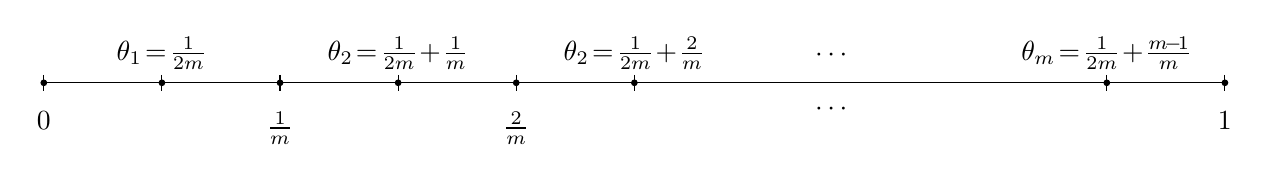
\begin{tikzpicture}[scale=1]
  % Draw horizontal axis
  \draw[-] (0,0) -- (15,0);
  % Mark positions
  \foreach \x/\name in {0/0, 3/$\frac{1}{m}$, 6/$\frac{2}{m}$, 15/1} {
    \draw (\x,0.1) -- (\x,-0.1) node[below=4pt] {\name};
    \filldraw[black] (\x,0) circle (1pt);
  }

  \foreach \x/\name in {1.5/$\theta_1\!=\!\frac{1}{2m}$, 4.5/$\theta_2\!=\!\frac{1}{2m}\!+\!\frac{1}{m}$, 7.5/$\theta_2\!=\!\frac{1}{2m}\!+\!\frac{2}{m}$, 13.5/$\theta_{m}\!=\!\frac{1}{2m}\!+\!\frac{m\!-\!1}{m}$} {
    \draw (\x,0.1) -- (\x,-0.1) node[above=4pt] {\name};
    \filldraw[black] (\x,0) circle (1pt);
  }
  \draw (10, 0) node[above=4pt] {$\cdots$};
  \draw (10, 0) node[below=4pt] {$\cdots$};

\end{tikzpicture}
\caption{Visualization of the discretization on the real line. Ground truth $Y_t$, forecasts $f(t)$ takes values in $\{0, 1/m, ..., 1\}$, and $\theta_i$ are between the grid points.} \label{fig:discretization}
\end{figure}

The following lemma shows that, to control regret uniformly over the class $S_\alpha$, it suffices to control regret on a finite collection of elementary scores $\{S_{\alpha,i}\}_{i=1}^m$. This reduction allows us to replace the original omniprediction objective over $S_\alpha$ with a tractable finite-dimensional problem. Proof is deferred to Appendix \ref{pf:discretize_single_q}.

\begin{lemma}[Discretizing all consistent losses] \label{lem:discretize_single_q}
  For any $\alpha \in (0,1) $, let $S_\alpha$ denote the class of scoring functions with representation \eqref{eq:elem_score_q} with $H([0,1]) \leq 1$.
\[
\sup_{f\in\cf, S\in S_\alpha} \E[S(p(X),Y)] - \E[S(f(X),Y)] 
=
\sup_{f\in\cf, i\in[m]} \E[S_{\alpha,i}(p(X),Y)] - \E[S_{\alpha,i}(f(X),Y)] 
\]
\end{lemma}





\subsection{Omniprediction algorithm and theoretical guarantee} \label{subsec:omni_single_q}
This subsection introduces the omniprediction algorithm that optimizes the losses for all consistent scoring rules for single quantile forecasts. Then, we prove a theoretical upper bound for the omniprediction error of the algorithm.

\begin{algorithm}[h]
  \caption{Single quantile level omniprediction} \label{alg:omni-twoplayer_online_q}
  \begin{algorithmic}[1]
  \State \textbf{Data:} Data stream $\{Y_t\}_{t=1}^T$, Grid size $m \in \mathbb{N}$, Learning rate $\eta > 0$, Base forecasters $\cf = \{f_b\}_{b=1}^{B}$.
  \State For $t=1$,$w_{ib}(t) = \frac{1}{mB}$, for all $i \in [m], b \in [B]$;

  \For{$t = 1, \ldots, T$}
    \State \textbf{1) Make prediction at time $t$}:
    \State $B_k := \sum_{i=1}^{k} \sum_{b=1}^B w_{ib}(t) - \sum_{i=1}^{m} \sum_{b=1}^B w_{ib}(t) \one(\theta_i < f_b(t))$, $\quad k^* = \max\{k: B_k \leq 0\}$
      \State \textbf{Output}
      \makebox[0pt][l]{$\displaystyle
          \hat{P}_t = \frac{B_{k^*+1}}{B_{k^*+1} + |B_{k^*}|}\delta_{\frac{k^*}{m}} +
          \frac{|B_{k^*}|}{B_{k^*+1} + |B_{k^*}|}\delta_{\frac{k^*+1}{m}}$
      } \vspace{-0.1cm}\\
      \State \textbf{2) Update the weights for each $S_{\theta_i}$ and $f_r$}:
          \State $w_{ib}(t+1) = \frac{w_{ib}(t) \exp\bigl(\eta \big(\mathbb{E}_{p \sim \hat{P}_t}[S_{\alpha, i}(p, Y_t)] 
          - S_{\alpha, i}(f_b(t), Y_t)\big)\bigr)}{\sum_{i,b} w_{ib}(t) \exp\bigl(\eta \big(\mathbb{E}_{p \sim \hat{P}_t}[S_{\alpha, i}(p, Y_t)] 
          - S_{\alpha, i}(f_b(t), Y_t)\big)\bigr)}, \quad \forall i \in [m], b \in [B];$ \vspace{-0.1cm}\\
  \EndFor
  \end{algorithmic}
\end{algorithm}



The first part of the algorithm is to produce a prediction at time $t$. Letting $\Delta_m$ denote the set of probability distributions over $\{0, \frac{1}{m}, \frac{2}{m}, ...,1\}$, the prediction $\hat{P}_t$ is computed as the minimax solution to the following program:
\begin{align}\label{eq:minimax_q}
  \hat{P}_t = \arg\min_{P \in \Delta_m} \max_{P_y \in \Delta_m} \sum_{i=1}^{m} \sum_{b=1}^B w_{ib} \,\E_{p\sim P, Y \sim P_y}[S_{\alpha,i}(p,Y) - S_{\alpha,i}(f_b(t),Y)] 
\end{align}
% to obtain a single quantile level forecast version of minimax program solution \eqref{eq:omni-twoplayer-minimax} in Algorithm \ref{alg:omni-twoplayer}.


% Now, we denote forecasts $\{\hat{f}_{\theta_i}\}_{i=0}^{m-1}$ be the forecast that minimizes the losses $\{S_{\alpha, \theta_i}\}_{i=0}^{m-1}$.

Following proposition provides a closed form solution to the minimax program \eqref{eq:minimax_q}, which is incorporated in Algorithm \ref{alg:omni-twoplayer_online_q}, by utilizing the structure of $S_{\alpha, i}$ losses. The proof is deferred to Appendix \ref{pf:minimax_sol_single_q}.

\begin{prop} \label{prop:minimax_sol_single_q}\todo{To add special care on $k^*=m$ case} Define $B_k := \sum_{i=1}^{k} \sum_{b=1}^B w_{ib} - \sum_{i=1}^{m} \sum_{b=1}^B w_{ib} \one(\theta_i < f_b(t))$ and let $k^* = \max\{k: B_k \leq 0\}$. Note that $B_{k^*} \leq 0$ and $B_{k^*+1}>0$. Then, 
\begin{align*}
P^* = \frac{B_{k^*+1}}{B_{k^*+1} + |B_{k^*}|}\delta_{\frac{k^*}{m}} + \frac{|B_{k^*}|}{B_{k^*+1} + |B_{k^*}|}\delta_{\frac{k^*+1}{m}} 
\quad\text{and}\quad
P_y^* = \alpha \delta_0 + (1-\alpha) \delta_1 
\end{align*}
solves equation \eqref{eq:minimax_q}.
\end{prop}

Now, we present the omniprediction error bound for Algorithm \ref{alg:omni-twoplayer_online_q}. The proof is deferred to Appendix \ref{pf:omni-twoplayer_online_q}.

\begin{theorem} \label{thm:omni-twoplayer_online_q}
  For a quantile level $\alpha \in (0,1)$, let $S_\alpha$ denote the class of scoring functions with representation \eqref{eq:elem_score_q} with $H(\R) = 1$ (the set of \textit{all} scoring functions that are consistent for the $\alpha$-level quantile functional under mild regularity conditions). Consider base forecasters $\{f_b\}_{b=1}^B$ that provide $\alpha$-level quantile forecasts $f_b(t)$ at each time step $t \in [T]$. With the target values $Y_t$, forecaster predictions $f_b(t)$ for $t \in [T], b \in [B]$ each taking values in a uniform grid of size $m$, and the learning rate $\eta = \sqrt{\frac{\log mB}{T}}$, the output $\hat{P}_t$ from Algorithm \ref{alg:omni-twoplayer_online_q} achieves the following omniprediction error:
  \begin{align*}
  \sup_{S \in S_\alpha,\, b \in [B]} \frac{1}{T} \sum_{t=1}^T \E_{p \sim \hat{P}(t)} [S(p, Y_t)] - \E[S(f_b(t), Y_t)]
  \leq 2\left(\sqrt{\frac{\log mB}{T}}\right)
  \end{align*}
\end{theorem}

